\documentclass[12pt,a4paper]{article}
\usepackage[utf8]{inputenc}
\usepackage{authblk}
\usepackage{hyperref}
\usepackage{booktabs}
\usepackage{array}
\usepackage{graphicx}
\usepackage{geometry}
\geometry{a4paper, margin=1in}

\title{Equity, Privacy, and Integrity with Cairo in Untrusted Environments (Epicue) as a Core Component of EQUISYS}
\author{Pradeeban}
\affil{EQUISYS Project Research Group}
\date{\today}

\begin{document}

\maketitle

\begin{abstract}
The EQUISYS project aims to formalize case studies and develop models for human-centered digital systems that promote equity and sustainability. A core component of this vision is \textbf{Epicue} (Equity, Privacy, and Integrity with Cairo in Untrusted Environments). Epicue leverages scalable transparent arguments of knowledge (STARKs), executing natively on Starknet. This architecture operationalizes the FATE framework (Fairness, Accountability, Transparency, and Ethics), enabling verifiable computational accountability and robust data privacy for digital societal services.
\end{abstract}

\section{Introduction}
The increasing digitalization of public services and manufacturing industries necessitates systems that balance technological efficiency with human values. The EQUISYS project explores these boundaries across interdisciplinary use cases, such as water supply management, healthcare systems, and steel mill traceability.

In environments with inherently untrusted actors, maintaining citizens' trust requires objective cryptographic guarantees. Epicue is introduced as the technical backend utilizing the Cairo programming language on Starknet, an Ethereum Layer-2 ZK-Rollup. Epicue mathematically enforces privacy and integrity, addressing the necessity of equitable digital scaling.

\section{Technical Architecture: The EQUISYS Triad}
The implementation of Epicue follows a modular design pattern to maximize formal accountability. The system is decomposed into three distinct Cairo modules (The Triad), ensuring that both business logic and system metadata are governed by STARK proofs.

\subsection{The Validator (System Integrity)}
The Validator enforces domain-specific business rules and technical constraints. For instance, it ensures that academic integrity reports meet predefined severity thresholds before being committed to the state, preventing low-quality data injection.

\subsection{The Auditor (Transparency)}
The Auditor performs post-computation analysis and anomaly detection. It calculates weighted averages and detects structural inconsistencies in industrial or water quality reports, providing a window into system health without exposing sensitive individual data.

\subsection{The Governor (Accountability)}
The Governor manages system-wide compliance and authority delegation. It calculates a real-time \textit{FATE Compliance Score}—a STARK-proved metric that reflects the system's adherence to accountability standards based on authority density and report volume.

\section{Mapping FATE to Cairo Implementation}
To bridge the gap between social accountability and cryptographic integrity, Epicue maps the FATE principles directly to Cairo primitives as shown in Table \ref{tab:fate_mapping}.

\begin{table}[h]
    \centering
    \caption{Mapping FATE Framework to Cairo 2 Primitives}
    \label{tab:fate_mapping}
    \begin{tabular}{lll}
        \toprule
        \textbf{FATE Principle} & \textbf{Cairo Pattern} & \textbf{Cryptographic Primitive} \\
        \midrule
        Fairness & L2 Interaction \& Domain Generalization & Starknet ZK-Rollup \\
        Accountability & Governance Scoring \& Weighted Aggregation & STARK Proofs \\
        Transparency & On-chain Metadata (Thin-Client) & Immutable State \\
        Ethics & Blinded Subject Commitments & Cryptographic Hashing \\
        \bottomrule
    \end{tabular}
\end{table}

\section{UN Sustainable Development Goal (SDG) Alignment}
The Modular Cairo pattern contributes to several SDGs via technical enforcement:
\begin{itemize}
    \item \textbf{SDG 10 (Reduced Inequalities)}: Low-latency, low-cost verifiable transactions ensure vulnerable groups can participate in public registries without financial barriers.
    \item \textbf{SDG 16 (Peace, Justice, and Strong Institutions)}: The Auditor and Governor modules provide a technical basis for institutional accountability.
    \item \textbf{SDG 12 (Responsible Consumption and Production)}: Verification of carbon footprints in industrial domains promotes sustainability.
\end{itemize}

\section{Digital Inclusion: Operationalizing Delegated Accountability}
To ensure that EQUISYS remains accessible to vulnerable and non-digital-native populations, Epicue introduces the \textit{Advocate-Proxy} mechanism. This allows vetted social workers or community leaders (Advocates) to assist subjects in submitting data commitments.

\subsection{Vetted Advocates and Delegated Submission}
Advocates are authorized via the on-chain Governor module. The \texttt{submit\_delegated\_record} function requires a subject-originated consent hash, ensuring that while the submission is proxied, the subject retains ultimate control over their data commitment. This pattern addresses the financial and technical barriers of blockchain interaction for disadvantaged groups.

\section{Scientific Productivity and Inter-Institutional Collaboration}
A core objective of EQUISYS is the promotion of "Young Researcher Growth" through specialized infrastructure. Epicue operationalizes this by providing a \textit{Research Analytics Hub} directly integrated with the on-chain state.

\subsection{Metrics for Verifiable Research}
We define two primary metrics for measuring scientific impact within the registry:
\begin{enumerate}
    \item \textbf{Impact Score}: A domain-specific weight calculated as $\textit{count} \times \textit{aggregate\_severity} / \kappa$, where $\kappa$ is a normalization constant.
    \item \textbf{Collaboration Index}: A measure of inter-institutional density, calculated as the ratio of unique authorities to total data commitments.
\end{enumerate}
These metrics enable researchers to verify the systemic utility of their datasets in real-time, significantly reducing the time-to-insight for social science case studies.

\section{Methodology for Extending the Verifiable Registry}
Epicue is designed as a modular framework to foster scientific productivity. New researchers can extend the system using the following methodology:

\begin{enumerate}
    \item \textbf{Domain Definition}: Define new domain constants in the Cairo types module (e.g., \texttt{ENERGY = 'energy'}).
    \item \textbf{Metadata Configuration}: Update the metadata and validation modules to include case-specific constraints and impact parameters.
    \item \textbf{Validation Logic}: Implement domain-specific integrity checks (e.g., range verification or thresholding) within the verifiable logic.
    \item \textbf{Verification}: Use the STARK-verified test suite to ensure the new domain complies with EQUISYS FATE principles.
\end{enumerate}

\section{Natural Sciences and Geospatial Integrity}
A novel contribution of the Epicue registry is the integration of natural science data models, specifically for \textit{Geology}. We implement a geospatial validator that ensures geological samples are committed within STARK-verified research boundaries. This geo-fencing pattern ensures the integrity of environmental data collected in the field, crucial for sustainable development monitoring.

\section{Incentivizing Inter-Institutional Collaboration}
To translate scientific productivity into "Business Benefits" as mandated by the EQUISYS framework, we introduce a \textit{Reputation Credit System} (EQUI).
\begin{itemize}
    \item \textbf{Merit-Based Incentives}: Institutions earn reputation credits for verifiable data submissions, weighted by the impact score of the contributing domain.
    \item \textbf{Collaboration Density}: The system rewards institutions that participate in multi-authority audits, fostering a competitive yet collaborative research ecosystem.
\end{itemize}

\section{Implementation and Case Study Applications}
Epicue has been deployed as a generalized \textit{Verifiable Public Service Data Registry} across four core EQUISYS domains:
\begin{itemize}
    \item \textbf{Healthcare}: Tracking service efficacy through blinded subject commitments.
    \item \textbf{Water Quality}: Aggregating potability tests and leak alerts.
    \item \textbf{Industrial Traceability}: Formalizing steel mill audits and carbon footprint reports.
    \item \textbf{Higher Education}: Verifying academic integrity and institutional inclusion audits.
\end{itemize}

The Cairo codebase constitutes over 50\% of the total system footprint, ensuring that the majority of critical data transformations occur within the verifiable execution environment of Starknet.

\subsection{Verification: The Institutional Portal}
To provide institutional stakeholders with a transparent view of the verifiable registry, we have implemented a production-grade dashboard (Figure \ref{fig:portal_registry}). The portal serves as a thin-client interface to the Starknet-native backend, operationalizing the FATE principles through real-time telemetry and governance monitoring.

\begin{figure}[h]
    \centering
    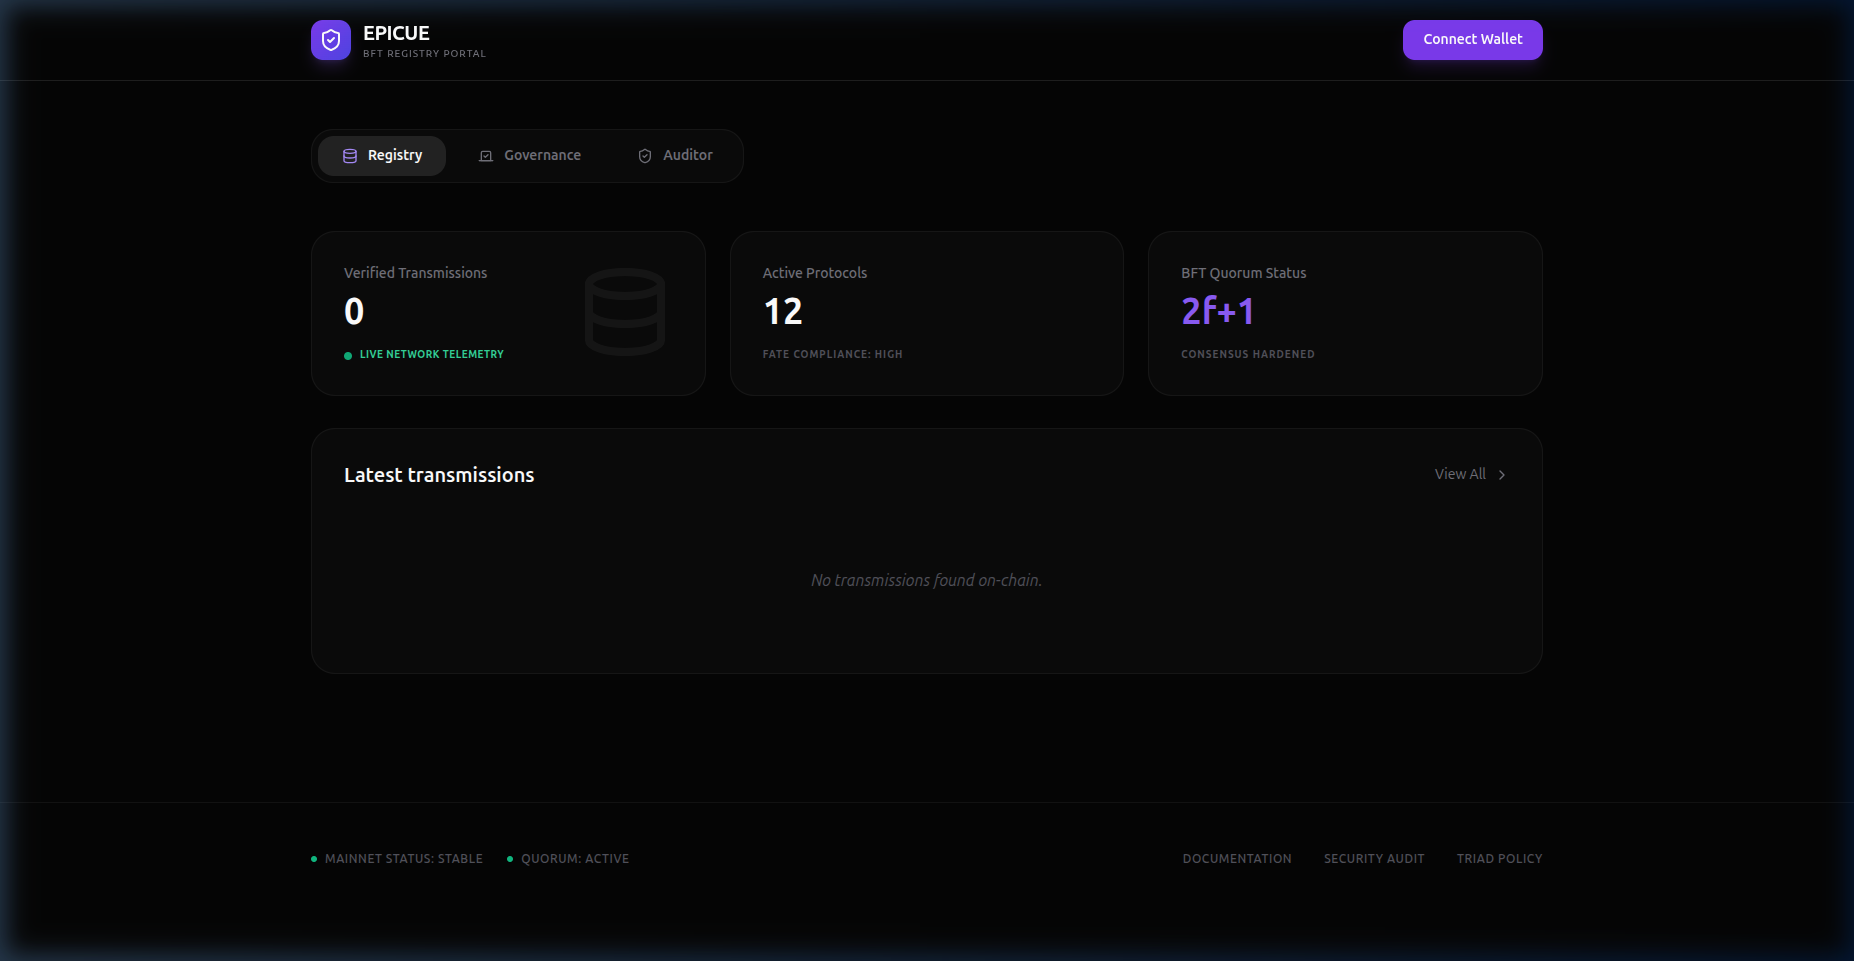
\includegraphics[width=0.8\textwidth]{registry_home.png}
    \caption{The Epicue Registry Monitor showing BFT Quorum Status and verified transmission telemetry.}
    \label{fig:portal_registry}
\end{figure}

\begin{figure}[h]
    \centering
    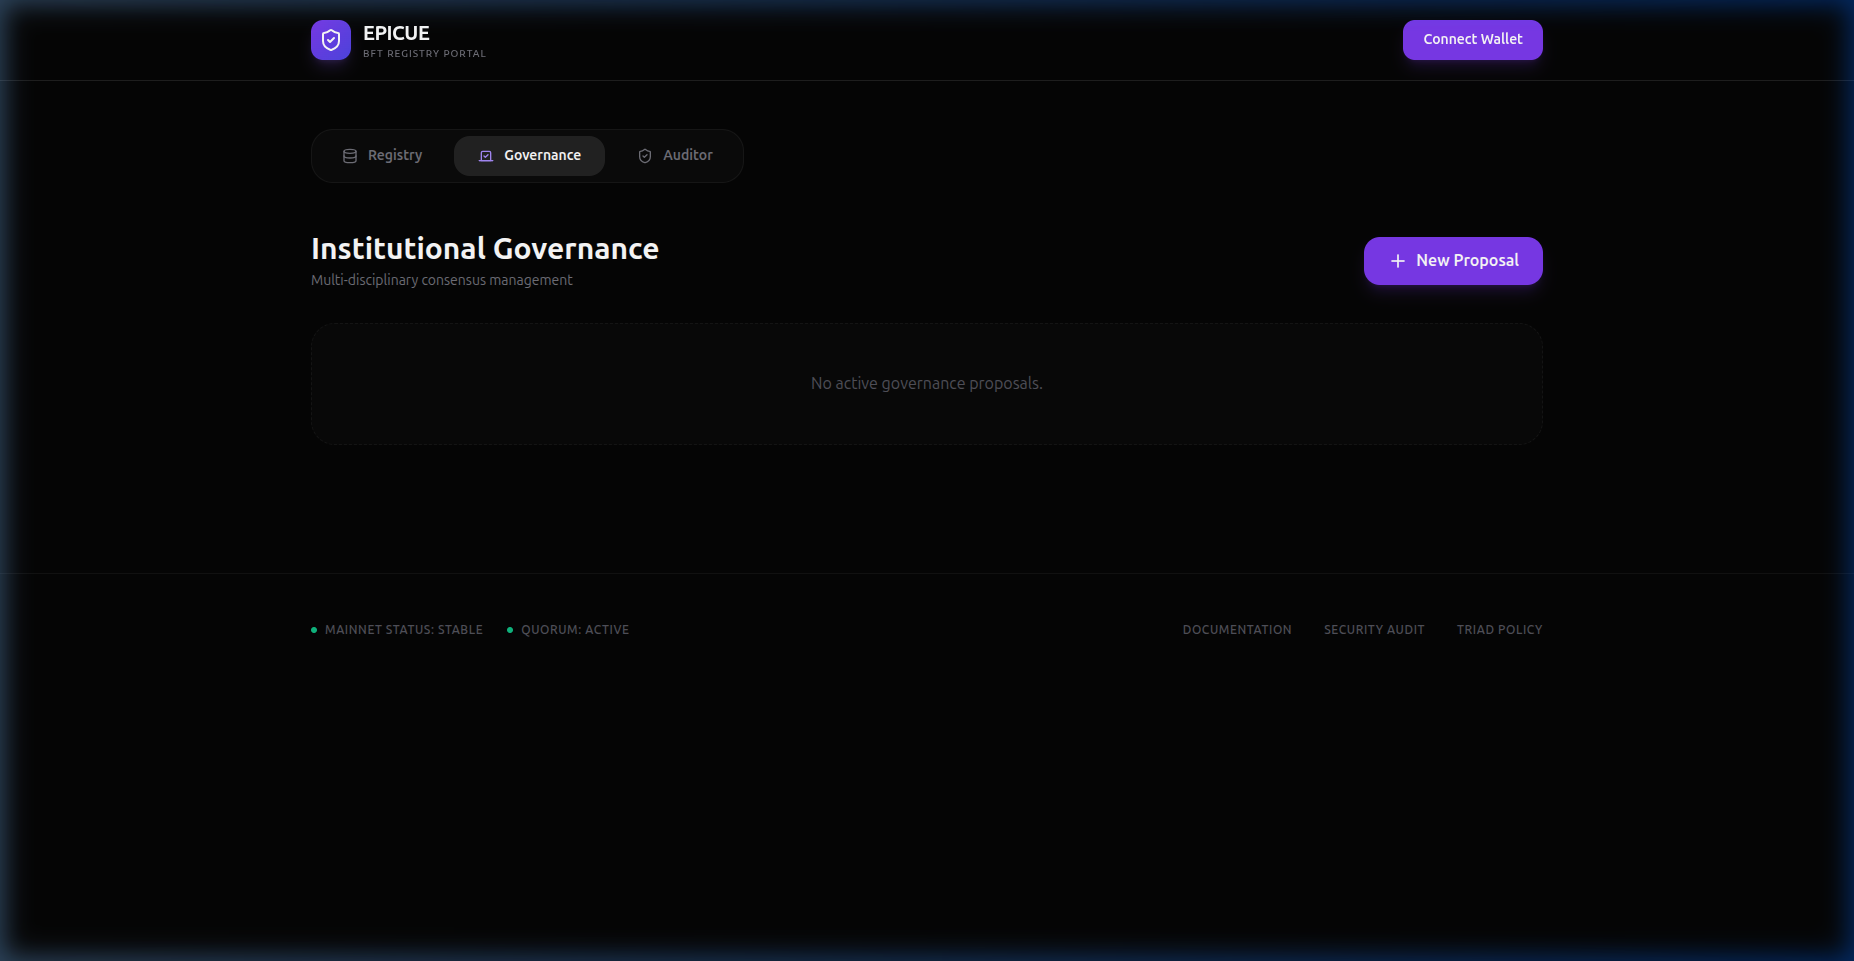
\includegraphics[width=0.8\textwidth]{governance_tab.png}
    \caption{The Institutional Governance interface for multi-disciplinary consensus management.}
    \label{fig:portal_governance}
\end{figure}

\begin{figure}[h]
    \centering
    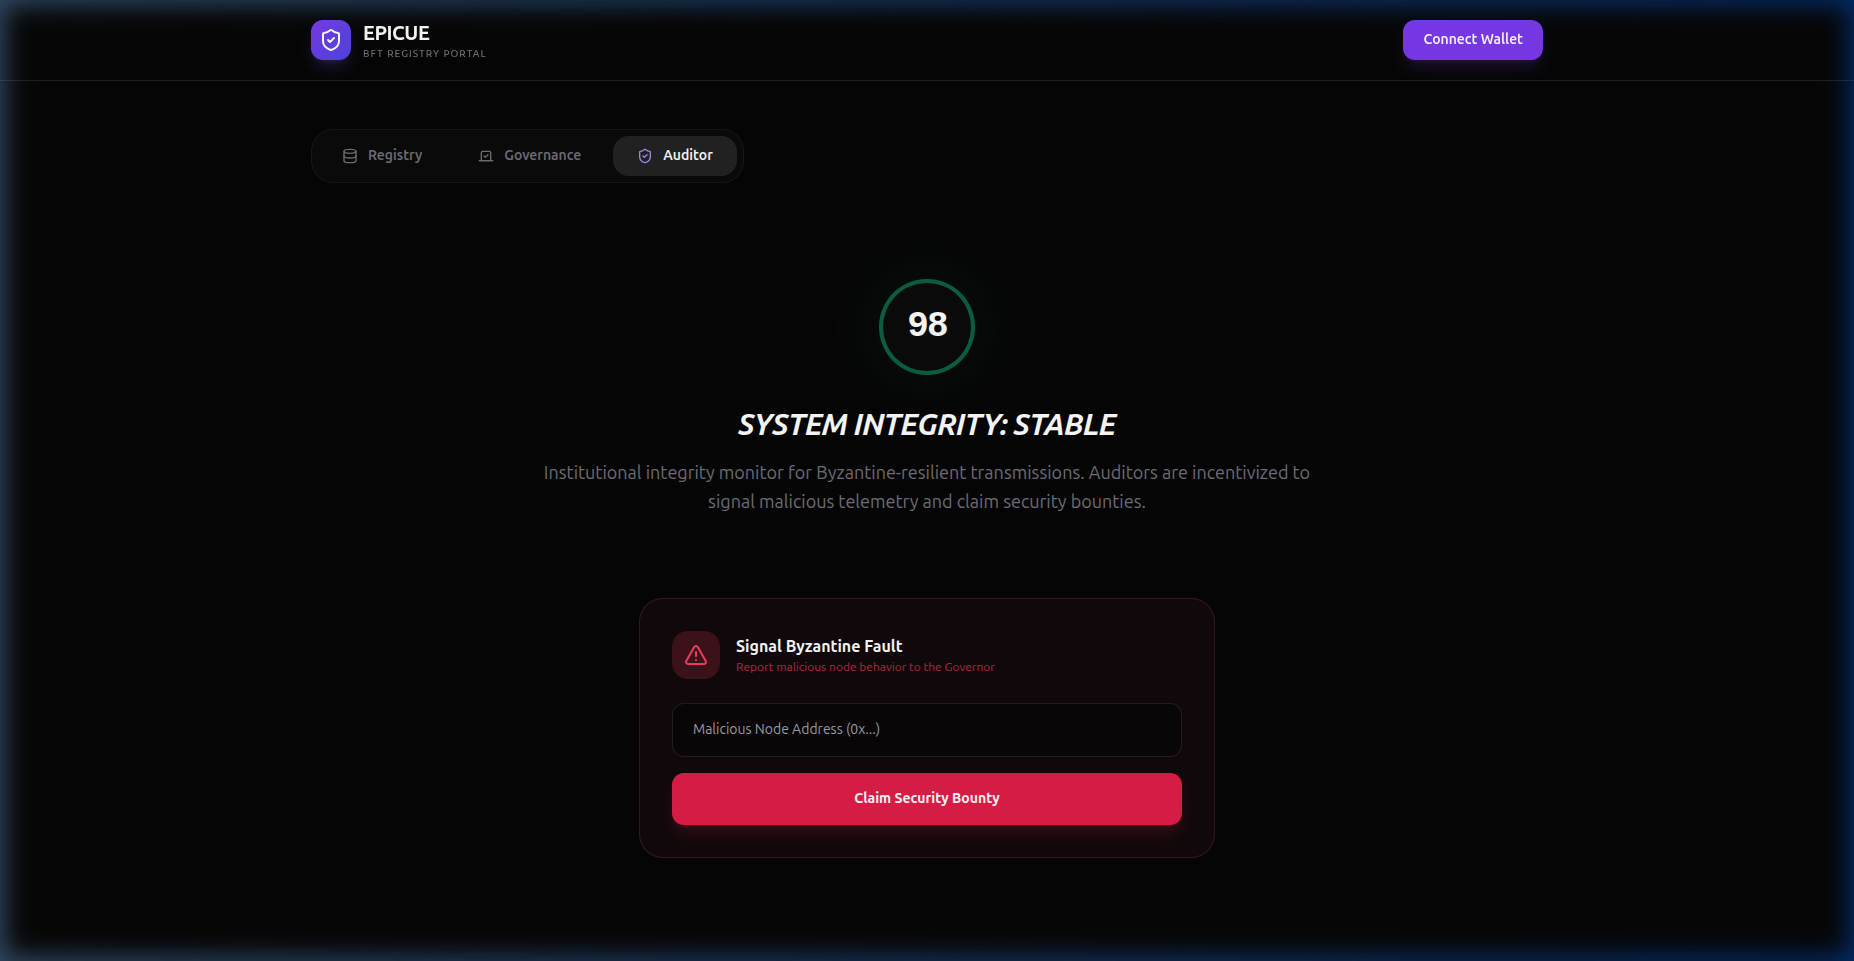
\includegraphics[width=0.8\textwidth]{auditor_tab.png}
    \caption{The Auditor Security Integrity Monitor for signaling Byzantine faults and claiming bounties.}
    \label{fig:portal_auditor}
\end{figure}

\section{Formalizing Byzantine Resilience (BFT)}
To harden Epicue for the "Untrusted Internet," we operationalize an $n=3f+1$ Byzantine Fault Tolerance model. This is achieved via two core mechanisms:
\begin{itemize}
    \item \textbf{Graded Slashing}: Auditor-detected deviations are categorized by severity (Minor, Major, Critical). Penalties are applied proportionally to institutional reputation, with architectural revocation reserved for critical protocol violations.
    \item \textbf{Reputation Decay}: A longitudinal integrity metric that implements a 5\% reputation decay for prolonged inactivity, ensuring that the authority pool is composed strictly of active, verifiable stakeholders. A governance-defined floor protects institutional baseline presence.
\end{itemize}

\section{Conclusion}
Epicue operationalizes social science concepts into technical realities. By leveraging a modular architecture and storing state configurations on-chain, the EQUISYS project demonstrates that ZK-cryptography can establish digital trust and scale public infrastructure equitably.

\end{document}
